

\subsection{SSL vs. TLS}
SSL (Secure Sockets Layer) und TLS (Transport Layer Security) sind Protokolle, die Verschlüsselung und Authentifizierung zwischen zwei Kommunikationspartnern bieten. Die beiden Begriffe SSL und TLS werden umgangssprachlich oft als zwei verschiedene Techniken dargestellt, obwohl TLS eine Weiterentwicklung von SSL ist. SSL v3 ist die Basis von TLS 1.0. \\
Aufgrund des Alters und einiger Sicherheitslücken wird SSL als unsicher angesehen und soll nicht mehr verwendet werden. Die aktuellste gefundene Lücke ist POODLE\footnote{SIcherheitslücke in SSL v3}, welche das Auslesen von Informationen aus einer verschlüsselten Übertragung erlaubt. Die Weiterentwicklungen TLS 1.1 und 1.2 sind deutlich sicherer und beheben einige Sicherheitslücken. So schützt die richtige Implementierung von TLS 1.2 auch vor den BEAST\footnote{Sicherheitslücke in TLS v1.0} Angriffsmethoden.\\

\subsection{Vor- und Nachteile TLS}
Da TLS auf der Transportschicht aufsetzt kann jedes höhere Protokoll darüber übertragen werden, somit ist die Verschlüsselung unabhängig von der genutzten Anwendung. \\
	Der größte Nachteil besteht darin, dass der Verbindungsaufbau serverseitig sehr rechenintensiv ist. Die Verschlüsselung selbst nimmt, abhängig vom Algorithmus, nur noch wenig Rechenleistung in Anspruch. \\

\subsection{TLS Handshake}
1. Client Hello\\
Übertragung von Verschlüsselungsinformationen vom Client an den Server, wie TLS Version oder Verschlüsselungsmöglichkeiten\\
2. Server Hello \\
Server sendet seine Informationen und legt Verschlüsselung fest. \\
3. Server Key Exchange\\
Server sendet seine Identität in Form seines Zertifikats. \\
4. Client Key Exchange\\
Client legt seinen Pre-Shared-Key fest und überträgt ihn verschlüsselt mit dem public Key des Servers.\\
5. Change Cipher Spec\\
Aus dem PSK wird ein Master-Secret generiert, mit welchem die folgenden Übertragung abgesichert wird. \\
6. Application Data\\
Übertragung der Daten. \\

\subsection{StartTLS}
Eine Variante von TLS ist das sogenannte STARTTLS, bei dem zuerst ein unsicheres 'hello' an den Server gesendet wird. Falls im Anschluss eine Verbindung erfolgreich Zustande kommt, wird zur sicheren Übertragung gewechselt. \\
Im ersten Versuch der Server-Client-Kommunikation in diesem Projekt wurden die Daten direkt zwischen Sockets übertragen. Im folgenden Ausschnitt ist der Wechsel zur Verschlüsselung sehr gut erkennbar: 
\begin{lstlisting}[caption = Starttls - Wechsel zur Verschlüsselung, language=python, frame=single, breaklines=true,columns=fullflexible, commentstyle=\color{gray}\upshape, captionpos=b, numbers = left]
if line == "STARTTLS":
	print "-- Switching to TLS"
	self.sendLine('READY')
	ctx = ServerTLSContext(
		privateKeyFileName='./certs/server.key',
		certificateFileName='./certs/server.crt',
			)
	self.transport.startTLS(ctx, self.factory)
\end{lstlisting}
Der vollständige Code ist im Commit unter \url{https://github.com/hoedding/Studienarbeit-Anwendung/commit/b52d056f55a9d65b9115ead2d2a2c0a549b366b6} zu finden

\subsection{Server Zertifikat}
Für die Verschlüsselung der Übertragung zwischen Server und Client ist ein Server-Zertifikat notwendig. Dieses wird mit OpenSSL in der neuesten Version generiert. \\
1. Private Key erzeugen
\begin{lstlisting}[caption =private Key, language=python, frame=single, breaklines=true,columns=fullflexible, commentstyle=\color{gray}\upshape, captionpos=b, numbers = left]
openssl genrsa -des3 -out server.key 2048
\end{lstlisting}

2. Certificate Signing Request
\begin{lstlisting}[caption =Certificate Signing Request, language=python, frame=single, breaklines=true,columns=fullflexible, commentstyle=\color{gray}\upshape, captionpos=b]
openssl req -new -key server.key -out server.csr
\end{lstlisting}


3. Self Signed Certificate\\
Bei einem öffentlichen Server sollte das Zertifikat bei einer CA (Certificate Authority) signiert werden. \\
\begin{lstlisting}[caption =Self Signed Certificate, language=python, frame=single, breaklines=true,columns=fullflexible, commentstyle=\color{gray}\upshape, captionpos=b]
openssl x509 -req -days 1865 -in server.csr -signkey server.key -out server.crt
\end{lstlisting}

\subsection{Apple Zertifikat}
Um die Apple Push Notifications einzusetzen ist ein Apple-Developer Zertifikat notwendig, welches nur über das Apple-Developer Portal erzeugt werden kann. Hierfür muss eine App-Identität angelegt werden. Im Anschluss wird auf einem Apple-Gerät ein Signing-Request erstellt. Dieser wird in das Developer-Portal hochgeladen. Im Anschluss wird ein Zertifikat generiert. Dieses muss in das Verzeichnis 'certs' gelegt werden. \\
Zusätzlich ist auf dem System ein Apple-Root Zertifikat erforderlich.\\\\
Die Generierung von Zertifikaten im Developer-Portal ist nur mit gültiger Apple-Developer-Registrierung möglich.

\subsection{Wireshark Trace}
Im folgenden ist ein Trace eines TLS Handshakes zwischen einem Client und dem implementierten Server (mit Twisted Framework) auf dem Raspberry Pi zu sehen. \\
Die einzelnen Schritte des Handshakes sind sehr gut erkennbar.\\
\begin{figure}[h]
\begin{minipage}{\textwidth}
            \centering
            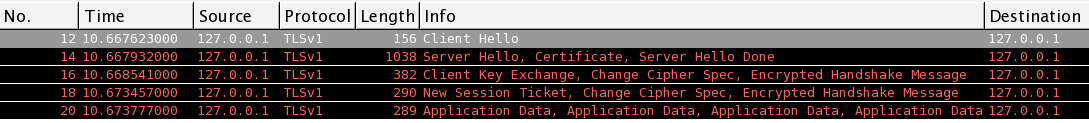
\includegraphics[width=\textwidth]{./data/wireshark.png}
            \caption{Wireshark Trace TLS Handshake}
        \end{minipage}
\end{figure}